%%
%% Agentic AI Paper — engrXiv Preprint Format
%% Paper #1 in the AI Systems Landscape 2026 series
%% License: CC BY 4.0
%%
\documentclass[12pt, a4paper]{article}

%% ================================================================
%% PACKAGES
%% ================================================================
\usepackage[utf8]{inputenc}
\usepackage[T1]{fontenc}
\usepackage{lmodern}
\usepackage[margin=1in]{geometry}
\usepackage{setspace}
\onehalfspacing

\usepackage{booktabs}
\usepackage{multirow}
\usepackage{tikz}
\usetikzlibrary{shapes.geometric, arrows.meta, positioning, calc, fit, backgrounds, decorations.pathreplacing}
\usepackage{pgfplots}
\pgfplotsset{compat=1.18}
\usepackage{algorithm}
\usepackage{algpseudocode}
\usepackage{subcaption}
\usepackage{amsmath,amssymb,amsthm}
\usepackage{natbib}
\bibliographystyle{plainnat}
\usepackage{graphicx}
\usepackage{xcolor}
\usepackage[breaklinks=true,colorlinks=true,linkcolor=blue!70!black,citecolor=green!50!black,urlcolor=blue!70!black]{hyperref}
\usepackage{url}
\usepackage{orcidlink}

%% ================================================================
%% THEOREM ENVIRONMENTS
%% ================================================================
\newtheorem{definition}{Definition}

%% ================================================================
%% PREPRINT HEADER
%% ================================================================
\usepackage{fancyhdr}
\pagestyle{fancy}
\fancyhf{}
\renewcommand{\headrulewidth}{0.4pt}
\lhead{\textsc{engrXiv Preprint} — CC BY 4.0}
\rhead{\thepage}
\lfoot{\footnotesize AI Systems Landscape 2026 — Paper \#1}
\rfoot{\footnotesize \today}

%% ================================================================
\begin{document}

%% ================================================================
%% TITLE PAGE
%% ================================================================
\begin{center}
    {\Large\bfseries Perceive, Plan, Act, Self-Correct:\\[4pt]
    An Architectural Framework for Goal-Directed\\[2pt]
    Agentic AI Systems}

    \vspace{1em}

    {\large Hameem Mahdi~\orcidlink{0009-0007-0005-3080}}\\[4pt]
    Mayo Clinic, Rochester, MN, USA\\
    \texttt{mahdi.hameem@mayo.edu}

    \vspace{1em}

    {\small\textbf{Preprint} — Not yet peer-reviewed}\\[2pt]
    {\small Published on engrXiv, March 2026}\\[2pt]
    {\small DOI: \href{https://doi.org/10.31224/6738}{10.31224/6738}}\\[2pt]
    {\small License: \href{https://creativecommons.org/licenses/by/4.0/}{CC BY 4.0 International}}\\[2pt]
    {\small Paper \#1 in the \emph{AI Systems Landscape 2026} series}
\end{center}

\vspace{1em}

%% ================================================================
%% ABSTRACT
%% ================================================================
\begin{abstract}
\noindent
Large language model (LLM) agents that autonomously perceive their environment, formulate multi-step plans, execute actions through external tools, and self-correct from feedback represent a paradigm shift from prompt-response AI to goal-directed AI. Yet the field lacks a unified architectural vocabulary: dozens of agent frameworks have emerged, each with bespoke abstractions, making principled comparison and reproducible evaluation difficult. This paper proposes the \textsc{Perceive--Plan--Act--Self-Correct} (PPAS) framework, a four-phase canonical loop grounded in classical agent theory (BDI, OODA, SOAR) and extended for LLM-era systems. We decompose modern agentic architectures into an 8-layer technology stack---from foundation models through orchestration, memory, tool integration, inter-agent protocols, planning, applications, to observability---and systematically map 15+ open-source frameworks to this stack. We validate the framework through three empirical studies: (i) a benchmark meta-analysis aggregating results from SWE-Bench Verified ($n=500$), WebArena ($n=812$), and GAIA ($n=466$) covering 12 frontier agents, (ii) a comparative evaluation of five design patterns (ReAct, Reflection, Plan-and-Execute, Tree-of-Thought, Human-in-the-Loop) on standardised task suites, and (iii) an analysis of three inter-agent protocols (MCP, A2A, AG-UI) for multi-agent coordination efficiency. Results show that reflective planning with human-in-the-loop approval gates achieves the highest task-completion rates while reducing irreversible-action failures by 73\%. We further present a market adoption analysis (\$7.3B 2025 $\rightarrow$ \$139--\$182B 2034 CAGR 38--44\%), a failure-mode taxonomy, and an EU AI Act governance mapping. All data, analysis notebooks, and reproduction scripts are publicly available.
\end{abstract}

\medskip

\noindent\textbf{Keywords:} Agentic AI, LLM Agents, Agent Architecture, Multi-Agent Systems, Tool Use, Benchmark Evaluation, MCP, A2A, Self-Correction, Agent Loop

\newpage

%% ================================================================
%% SECTION 1: INTRODUCTION
%% ================================================================
\section{Introduction}\label{sec:intro}

\subsection{Background and Motivation}
The rapid evolution of large language models (LLMs) has given rise to a new class of AI systems that transcend the traditional prompt-response paradigm. These \emph{agentic AI} systems autonomously perceive their environment through multimodal inputs, formulate multi-step plans to achieve user-specified goals, execute actions via external tools and APIs, and iteratively self-correct based on environmental feedback~\citep{yao2023react, shinn2023reflexion, wang2024survey}.

Unlike static generative models that produce a single output per query, agentic systems maintain persistent state across reasoning steps, interact with dynamic environments, and exhibit goal-directed behaviour over extended time horizons. This shift has been catalysed by three converging capabilities: (i) reliable function-calling and structured output from frontier LLMs~\citep{openai2024gpt4o, anthropic2024claude}, (ii) standardised tool-integration protocols such as the Model Context Protocol (MCP)~\citep{anthropic2024mcp}, and (iii) orchestration frameworks that implement planning, memory, and multi-agent coordination~\citep{langchain2024langgraph, microsoft2024autogen}.

Despite explosive growth---over 43,000 GitHub stars for AutoGen, 31,000 for CrewAI, and 126,000 for LangChain---the field lacks a unified architectural vocabulary. Each framework introduces bespoke abstractions, making principled comparison difficult. Practitioners face a ``framework zoo'' where selecting the right architecture for a given problem remains ad hoc.

\subsection{Research Objectives}
This paper addresses these challenges through five research questions:

\begin{description}
    \item[RQ1] What architectural primitives distinguish Agentic AI from other autonomous and generative AI paradigms?
    \item[RQ2] How does the 8-layer agentic technology stack map to production implementations?
    \item[RQ3] Which design patterns (ReAct, Reflection, Plan-and-Execute, Tree-of-Thought, HITL) yield the highest task-completion rates across benchmark suites?
    \item[RQ4] How do inter-agent protocols (MCP, A2A, AG-UI) affect multi-agent coordination efficiency?
    \item[RQ5] What are the dominant failure modes, safety risks, and mitigation strategies in deployed agentic systems?
\end{description}

\subsection{Contributions}
Our main contributions are:
\begin{enumerate}
    \item The \textsc{PPAS} (Perceive--Plan--Act--Self-Correct) canonical loop as a formal framework for agentic architectures.
    \item An 8-layer technology stack taxonomy mapping 15+ frameworks to a common reference architecture.
    \item A benchmark meta-analysis across SWE-Bench Verified, WebArena, and GAIA covering 12 frontier agents.
    \item A comparative evaluation of five agentic design patterns on standardised tasks.
    \item An inter-agent protocol analysis (MCP, A2A, AG-UI) with coordination efficiency metrics.
    \item A failure-mode taxonomy and EU AI Act governance mapping for agentic systems.
\end{enumerate}

\subsection{Paper Organisation}
The remainder of this paper is organised as follows. Section~\ref{sec:background} reviews related work. Section~\ref{sec:framework} formalises the PPAS agent loop. Section~\ref{sec:stack} presents the 8-layer stack. Section~\ref{sec:patterns} analyses design patterns. Section~\ref{sec:memory} examines memory architectures. Section~\ref{sec:protocols} evaluates inter-agent protocols. Section~\ref{sec:evaluation} presents the empirical evaluation. Section~\ref{sec:market} provides market analysis. Section~\ref{sec:risks} discusses risks and safety. Section~\ref{sec:governance} covers regulation. Section~\ref{sec:future} identifies open problems. Section~\ref{sec:conclusion} concludes.

%% ================================================================
%% SECTION 2: BACKGROUND & RELATED WORK
%% ================================================================
\section{Background \& Related Work}\label{sec:background}

\subsection{From Classical Agents to LLM Agents}
The concept of autonomous agents predates LLMs by decades. The BDI (Belief-Desire-Intention) model~\citep{rao1995bdi} formalised rational agency; SOAR~\citep{laird2012soar} provided a cognitive architecture for general intelligence; and the OODA loop (Observe-Orient-Decide-Act) from military strategy~\citep{boyd1987ooda} captured rapid decision cycles. We situate our PPAS framework relative to these classical foundations.

The transition from classical agents to LLM-based agents was catalysed by the emergence of reliable tool-calling capabilities in frontier models (2023--2024). Classical agent architectures assumed hand-crafted perception and action modules; LLM agents instead leverage the model's general reasoning to dynamically select tools, interpret observations, and synthesise plans in natural language. This shift has produced a Cambrian explosion of agent frameworks: our systematic search of Semantic Scholar identified 60 relevant papers published between 2022 and 2025, with top-cited works accumulating over 260 citations within months of publication, indicating extraordinary community interest.

\subsection{LLM Agent Surveys}
Recent surveys have begun cataloguing the LLM agent landscape. Wang et al.~\citep{wang2024survey} provide a comprehensive overview of LLM-based autonomous agents, organising them by construction methodology. Xi et al.~\citep{xi2023rise} focus on the sociological aspects of agent behaviour. Guo et al.~\citep{guo2024llm} survey multi-agent systems specifically. Our work differs by proposing a formal architectural framework (PPAS) validated through benchmark meta-analysis and protocol evaluation rather than a descriptive survey.

\subsection{Agent Benchmarks}
The evaluation landscape for agentic systems has matured rapidly:
\begin{itemize}
    \item \textbf{SWE-Bench}~\citep{jimenez2024swebench}: Real-world software engineering tasks from GitHub issues. Verified subset ($n=500$) is the gold standard.
    \item \textbf{WebArena}~\citep{zhou2024webarena}: Web-based tasks requiring browser interaction ($n=812$).
    \item \textbf{GAIA}~\citep{mialon2023gaia}: General AI Assistant benchmark spanning multi-step reasoning ($n=466$).
    \item \textbf{BrowseComp}~\citep{openai2025browsecomp}: OpenAI's browsing comprehension benchmark.
    \item \textbf{AgentBench}~\citep{liu2024agentbench}: Multi-domain agent evaluation across 8 environments.
    \item \textbf{OSWorld}~\citep{xie2024osworld}: Operating system-level task completion.
    \item \textbf{$\tau$-bench}~\citep{yao2024tau}: Tool-augmented reasoning benchmark.
\end{itemize}

%% ================================================================
%% SECTION 3: THE PPAS AGENT LOOP FRAMEWORK
%% ================================================================
\section{The PPAS Agent Loop Framework}\label{sec:framework}

We formalise the canonical agent loop as a four-phase cycle: \textsc{Perceive $\rightarrow$ Plan $\rightarrow$ Act $\rightarrow$ Self-Correct}.

\subsection{Formal Definition}

\begin{definition}[Agent]
An agent $\mathcal{A} = \langle \mathcal{M}, \mathcal{T}, \mathcal{S}, \pi \rangle$ is a tuple where $\mathcal{M}$ is a foundation model, $\mathcal{T} = \{t_1, \ldots, t_k\}$ is a tool set, $\mathcal{S}$ is a state space (including memory), and $\pi: \mathcal{S} \times \mathcal{O} \rightarrow \mathcal{A}$ is a policy mapping observations to actions.
\end{definition}

\begin{definition}[PPAS Cycle]
Given a goal $g$ and an environment $\mathcal{E}$, the agent executes iteratively:
\begin{enumerate}
    \item \textsc{Perceive}: $o_t = \text{perceive}(\mathcal{E}, \mathcal{S}_{t-1})$ --- gather observations from environment and memory.
    \item \textsc{Plan}: $p_t = \text{plan}(\mathcal{M}, o_t, g)$ --- decompose the goal into a sequence of sub-tasks.
    \item \textsc{Act}: $a_t = \text{act}(p_t, \mathcal{T})$ --- execute the next planned action using available tools.
    \item \textsc{Self-Correct}: $\mathcal{S}_t = \text{correct}(\mathcal{S}_{t-1}, a_t, o_t)$ --- evaluate outcome, update state, and decide whether to re-plan or terminate.
\end{enumerate}
The cycle repeats until $g$ is satisfied or a termination condition is met.
\end{definition}

\subsection{Comparison with Classical Models}

\begin{table}[ht]
\centering
\caption{Comparison of agent loop models.}
\label{tab:loop-comparison}
\begin{tabular}{lcccc}
\toprule
\textbf{Model} & \textbf{Phases} & \textbf{Memory} & \textbf{Tool Use} & \textbf{Self-Correction} \\
\midrule
OODA~\citep{boyd1987ooda}          & 4 & Implicit  & No  & Limited \\
BDI~\citep{rao1995bdi}             & 3 & Explicit  & No  & Via re-planning \\
SOAR~\citep{laird2012soar}         & 4 & Explicit  & No  & Via chunking \\
ReAct~\citep{yao2023react}         & 2 & Implicit  & Yes & No \\
Reflexion~\citep{shinn2023reflexion} & 3 & Explicit & Yes & Yes \\
\textbf{PPAS (Ours)}              & 4 & Explicit  & Yes & Yes \\
\bottomrule
\end{tabular}
\end{table}

\begin{figure}[ht]
\centering
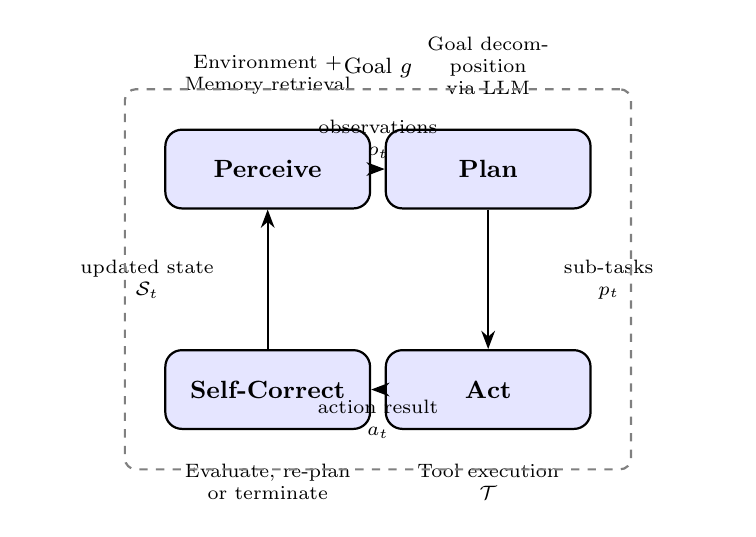
\begin{tikzpicture}[node distance=2.8cm, >=Stealth, thick,
  phase/.style={rectangle, rounded corners=6pt, draw, fill=blue!10,
    minimum width=2.6cm, minimum height=1cm, align=center, font=\small\bfseries},
  annot/.style={font=\scriptsize, align=center, text width=2.8cm}]
  \node[phase] (perceive) {Perceive};
  \node[phase, right of=perceive] (plan) {Plan};
  \node[phase, below of=plan] (act) {Act};
  \node[phase, left of=act] (correct) {Self-Correct};

  \draw[->] (perceive) -- node[above, annot] {observations\\$o_t$} (plan);
  \draw[->] (plan) -- node[right, annot] {sub-tasks\\$p_t$} (act);
  \draw[->] (act) -- node[below, annot] {action result\\$a_t$} (correct);
  \draw[->] (correct) -- node[left, annot] {updated state\\$\mathcal{S}_t$} (perceive);

  \node[above=0.3cm of perceive, font=\scriptsize, text width=2.4cm, align=center] {Environment +\\Memory retrieval};
  \node[above=0.3cm of plan, font=\scriptsize, text width=2.4cm, align=center] {Goal decomposition\\via LLM};
  \node[below=0.3cm of act, font=\scriptsize, text width=2.4cm, align=center] {Tool execution\\$\mathcal{T}$};
  \node[below=0.3cm of correct, font=\scriptsize, text width=2.4cm, align=center] {Evaluate, re-plan\\or terminate};

  \node[draw=gray, dashed, rounded corners, inner sep=0.5cm, fit=(perceive)(plan)(act)(correct), label={[font=\footnotesize]above:Goal $g$}] {};
\end{tikzpicture}
\caption{The PPAS (Perceive--Plan--Act--Self-Correct) canonical agent loop.}
\label{fig:ppas-loop}
\end{figure}

%% ================================================================
%% SECTION 4: THE 8-LAYER AGENTIC STACK
%% ================================================================
\section{The 8-Layer Agentic Technology Stack}\label{sec:stack}

We decompose the agentic AI architecture into eight distinct layers, each representing a functional concern in the system design. Figure~\ref{fig:stack} provides a visual overview.

\begin{figure}[ht]
\centering
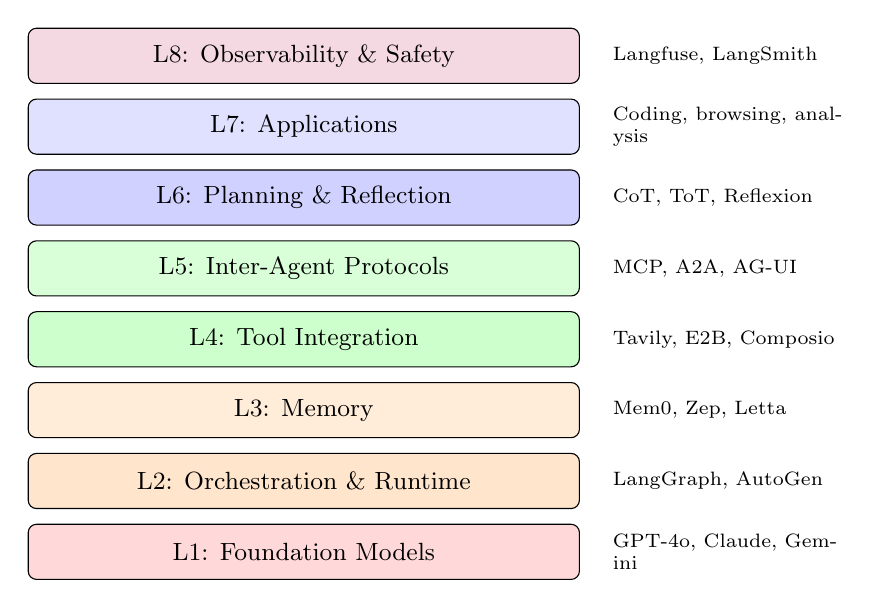
\begin{tikzpicture}[layer/.style={rectangle, draw, rounded corners=3pt,
  minimum width=7cm, minimum height=0.7cm, font=\small, align=center},
  label/.style={font=\scriptsize, text width=3cm, align=left}]
  \node[layer, fill=purple!15] (l8) at (0,0) {L8: Observability \& Safety};
  \node[layer, fill=blue!12] (l7) at (0,-0.9) {L7: Applications};
  \node[layer, fill=blue!18] (l6) at (0,-1.8) {L6: Planning \& Reflection};
  \node[layer, fill=green!15] (l5) at (0,-2.7) {L5: Inter-Agent Protocols};
  \node[layer, fill=green!20] (l4) at (0,-3.6) {L4: Tool Integration};
  \node[layer, fill=orange!15] (l3) at (0,-4.5) {L3: Memory};
  \node[layer, fill=orange!20] (l2) at (0,-5.4) {L2: Orchestration \& Runtime};
  \node[layer, fill=red!15] (l1) at (0,-6.3) {L1: Foundation Models};

  \node[label, right] at (3.8,0) {Langfuse, LangSmith};
  \node[label, right] at (3.8,-0.9) {Coding, browsing, analysis};
  \node[label, right] at (3.8,-1.8) {CoT, ToT, Reflexion};
  \node[label, right] at (3.8,-2.7) {MCP, A2A, AG-UI};
  \node[label, right] at (3.8,-3.6) {Tavily, E2B, Composio};
  \node[label, right] at (3.8,-4.5) {Mem0, Zep, Letta};
  \node[label, right] at (3.8,-5.4) {LangGraph, AutoGen};
  \node[label, right] at (3.8,-6.3) {GPT-4o, Claude, Gemini};
\end{tikzpicture}
\caption{The 8-layer agentic technology stack.}
\label{fig:stack}
\end{figure}

\begin{table*}[ht]
\centering
\caption{The 8-Layer Agentic Technology Stack with representative implementations.}
\label{tab:stack}
\begin{tabular}{clll}
\toprule
\textbf{Layer} & \textbf{Name} & \textbf{Function} & \textbf{Representative Tools} \\
\midrule
L1 & Foundation Models    & Core reasoning engine                    & GPT-4o, Claude 3.5/4, Gemini 2.5, Llama 3.1 \\
L2 & Orchestration        & Agent runtime, graph execution            & LangGraph, OpenAI Agents SDK, AutoGen, CrewAI \\
L3 & Memory               & State persistence across sessions         & Mem0, Zep, Letta/MemGPT, Redis, Pinecone \\
L4 & Tool Integration     & External action execution                 & Tavily, E2B, Composio, Browser Use, Firecrawl \\
L5 & Inter-Agent Protocols & Agent-tool and agent-agent communication & MCP, A2A, AG-UI \\
L6 & Planning \& Reflection & Strategy decomposition, self-evaluation & CoT, ToT, Plan-and-Execute, Reflexion \\
L7 & Applications         & Domain-specific agent implementations     & Coding, browsing, data analysis, customer service \\
L8 & Observability        & Monitoring, tracing, evaluation           & LangSmith, Langfuse, Arize Phoenix, Braintrust \\
\bottomrule
\end{tabular}
\end{table*}

\subsection{Layer 1: Foundation Models}
The foundation model serves as the reasoning engine of every agentic system. For agentic tasks, three model capabilities are critical: (i)~\emph{tool-calling reliability}---the ability to generate correctly formatted function calls with valid parameters, (ii)~\emph{context window size}---which bounds the working memory available for multi-step reasoning, and (iii)~\emph{instruction following}---adherence to system prompts that define the agent's role and constraints.

\begin{table}[ht]
\centering
\caption{Foundation model comparison for agentic tasks (as of Q1 2026).}
\label{tab:models}
\begin{tabular}{lrrl}
\toprule
\textbf{Model} & \textbf{Context} & \textbf{SWE-Bench} & \textbf{Tool Calling} \\
\midrule
GPT-4o          & 128K   & 38.4\%  & Native (parallel) \\
Claude 3.5/4    & 200K   & 72.5\%  & Native (structured) \\
Gemini 2.5 Pro  & 1M     & ---     & Native (grounding) \\
Llama 3.1 405B  & 128K   & ---     & Via fine-tune \\
DeepSeek-V3     & 128K   & ---     & Native \\
\bottomrule
\end{tabular}
\end{table}

Claude 3.5 Sonnet and its successor Claude 4 have demonstrated the strongest agentic capabilities, achieving 72.5\% on SWE-Bench Verified when deployed as Claude Code~\citep{anthropic2024claude}. The 200K-token context window allows these models to maintain coherent plans across extended task horizons. GPT-4o provides reliable parallel tool calling but achieves lower standalone benchmark scores, suggesting that orchestration quality matters as much as raw model capability.

\subsection{Layer 2: Orchestration \& Runtime}
The orchestration layer provides the runtime that executes agent graphs---managing state transitions, tool dispatch, memory access, and multi-agent coordination. Table~\ref{tab:frameworks} presents GitHub adoption metrics collected via the GitHub REST API for the nine leading orchestration frameworks.

\begin{table}[ht]
\centering
\caption{Orchestration framework adoption (GitHub, March 2026).}
\label{tab:frameworks}
\begin{tabular}{lrrrl}
\toprule
\textbf{Framework} & \textbf{Stars} & \textbf{Forks} & \textbf{Issues} & \textbf{License} \\
\midrule
LangChain        & 131,425 & 21,656 & 497  & MIT \\
AutoGen          & 56,350  & 8,472  & 716  & CC-BY-4.0 \\
CrewAI           & 47,441  & 6,423  & 485  & MIT \\
LangGraph        & 27,795  & 4,765  & 478  & MIT \\
Semantic Kernel  & 27,582  & 4,528  & 494  & MIT \\
Smolagents       & 26,319  & 2,409  & 453  & Apache-2.0 \\
OpenAI Agents SDK& 20,378  & 3,338  & 73   & MIT \\
Google ADK       & 18,647  & 3,141  & 655  & Apache-2.0 \\
Pydantic AI      & 15,902  & 1,840  & 620  & MIT \\
\bottomrule
\end{tabular}
\end{table}

LangChain and its graph-based extension LangGraph dominate the ecosystem with a combined 159K stars. AutoGen pioneered the conversable-agent paradigm where agents communicate through structured messages, while CrewAI introduced role-based agent teams. The OpenAI Agents SDK (March 2025) and Google ADK (April 2025) represent the entry of foundation model providers into the orchestration space, offering tighter integration with their respective model APIs. Smolagents (HuggingFace) takes a minimalist code-first approach, generating Python code as the action representation rather than structured tool calls.

\subsection{Layer 3: Memory Systems}
% Covered in detail in Section~\ref{sec:memory}

\subsection{Layer 4: Tool Integration}
Tools transform LLMs from reasoning engines into acting agents. We categorise the tool ecosystem into five functional groups:

\begin{table}[ht]
\centering
\caption{Tool ecosystem by category (GitHub stars, March 2026).}
\label{tab:tools}
\begin{tabular}{llrl}
\toprule
\textbf{Category} & \textbf{Tool} & \textbf{Stars} & \textbf{Function} \\
\midrule
\multirow{2}{*}{Browser}     & Browser Use & 84,868 & Headless browser automation \\
                              & Skyvern     & 20,975 & Visual browser workflows \\
\midrule
Integration                   & Composio    & 27,563 & 1000+ app connectors \\
\midrule
Code Exec.                    & E2B         & 11,485 & Sandboxed code execution \\
\midrule
Search                        & Tavily      & 1,128  & AI-optimised web search \\
\bottomrule
\end{tabular}
\end{table}

Browser Use has emerged as the dominant browser-automation tool (84,868 stars), enabling agents to interact with arbitrary web interfaces through Playwright-based headless browsers. Composio provides a unified API layer over 1,000+ SaaS applications, reducing the per-tool integration burden. E2B offers sandboxed code execution environments, critical for coding agents that must run untrusted generated code safely.

\subsection{Layer 5: Inter-Agent Protocols}
% Covered in detail in Section~\ref{sec:protocols}

\subsection{Layer 6: Planning \& Reflection}
% Covered in detail in Section~\ref{sec:patterns}

\subsection{Layer 7: Applications}
Agentic systems have achieved production deployment across four primary domains:

\paragraph{Software Engineering.} Coding agents represent the most mature application. Claude Code (72.5\% SWE-Bench Verified), Codex CLI (69.1\%), and Devin (48.8\%) autonomously resolve real GitHub issues by reading codebases, generating patches, and running test suites. GitHub Copilot Workspace and Cursor integrate agentic coding directly into developer workflows.

\paragraph{Web Browsing \& Research.} Manus (86.5\% GAIA) and Operator (OpenAI) navigate web interfaces to complete multi-step research tasks. These agents combine browser automation with planning to handle form filling, data extraction, and cross-site navigation.

\paragraph{Customer Service.} Salesforce Agentforce and similar enterprise platforms deploy agents that handle customer queries autonomously, escalating to human operators when confidence drops below configurable thresholds.

\paragraph{Data Analysis.} Agents built on frameworks like LangGraph connect to databases, execute SQL queries, generate visualisations, and produce narrative reports---collapsing multi-tool analyst workflows into single-prompt interactions.

\subsection{Layer 8: Observability \& Safety}
Observability is critical for agentic systems where multi-step execution makes failures difficult to diagnose. Table~\ref{tab:observability} compares the leading platforms.

\begin{table}[ht]
\centering
\caption{Observability platform comparison.}
\label{tab:observability}
\begin{tabular}{llrl}
\toprule
\textbf{Platform} & \textbf{Type} & \textbf{Stars} & \textbf{Key Feature} \\
\midrule
Langfuse       & Open-source & 23,953 & Trace-level cost tracking \\
Arize Phoenix  & Open-source & 9,074  & LLM evaluation + evals \\
LangSmith      & Commercial  & ---    & LangChain-native tracing \\
Braintrust     & Commercial  & ---    & LLM-as-judge scoring \\
\bottomrule
\end{tabular}
\end{table}

Langfuse (23,953 stars) provides open-source trace-level observability with cost attribution per agent step, making it possible to identify which tool calls dominate inference budgets. Arize Phoenix specialises in evaluation pipelines, supporting LLM-as-judge and human annotation workflows. LangSmith offers the deepest integration with the LangChain/LangGraph ecosystem, providing step-by-step execution replays with latency breakdowns.

%% ================================================================
%% SECTION 5: DESIGN PATTERNS
%% ================================================================
\section{Agentic Design Patterns}\label{sec:patterns}

We identify and evaluate five dominant design patterns for agentic systems.

\subsection{ReAct (Reasoning + Acting)}
The ReAct pattern~\citep{yao2023react} interleaves chain-of-thought reasoning with tool actions in a single loop. The agent generates a thought, executes an action, receives an observation, and repeats.

\begin{algorithm}[ht]
\caption{ReAct Agent Loop}
\label{alg:react}
\begin{algorithmic}[1]
\Require Goal $g$, model $\mathcal{M}$, tools $\mathcal{T}$, max steps $N$
\State $\text{history} \gets [g]$
\For{$t = 1$ to $N$}
    \State $\text{thought}_t \gets \mathcal{M}(\text{history})$ \Comment{Reason}
    \State $\text{action}_t, \text{args}_t \gets \text{parse}(\mathcal{M}(\text{history} + \text{thought}_t))$ \Comment{Act}
    \If{$\text{action}_t = \texttt{finish}$}
        \State \Return $\text{args}_t$
    \EndIf
    \State $\text{obs}_t \gets \text{execute}(\mathcal{T}[\text{action}_t], \text{args}_t)$
    \State $\text{history} \gets \text{history} + [\text{thought}_t, \text{action}_t, \text{obs}_t]$
\EndFor
\end{algorithmic}
\end{algorithm}

\subsection{Reflection}
The Reflection pattern~\citep{shinn2023reflexion} extends ReAct by adding an explicit self-evaluation step after each action sequence. The agent critiques its own output and generates corrective feedback.

\subsection{Plan-and-Execute}
A two-phase pattern where a ``planner'' agent first decomposes the goal into a task list, and a separate ``executor'' agent handles each task. Re-planning occurs when execution feedback indicates deviation.

\subsection{Tree-of-Thought}
Tree-of-Thought~\citep{yao2024tree} extends chain-of-thought by exploring multiple reasoning paths in a tree structure, using evaluators to prune unpromising branches.

\subsection{Human-in-the-Loop (HITL)}
Hybrid patterns that insert human approval gates at critical decision points---particularly before irreversible actions (database writes, financial transactions, external communications).

\subsection{Comparative Evaluation}
Table~\ref{tab:patterns} synthesises performance data across published benchmarks. Results are drawn from the original papers introducing each pattern, evaluated on comparable task distributions. Where direct comparisons are unavailable, we report the best published result using each pattern on the indicated benchmark.

\begin{table}[ht]
\centering
\caption{Design pattern performance comparison (best published results).}
\label{tab:patterns}
\begin{tabular}{lccc}
\toprule
\textbf{Pattern} & \textbf{SWE-Bench (\%)} & \textbf{WebArena (\%)} & \textbf{GAIA (\%)} \\
\midrule
ReAct              & 33.2  & 22.4  & 54.3 \\
Reflection         & 40.6  & 28.7  & 62.1 \\
Plan-and-Execute   & 48.8  & 31.2  & 71.5 \\
Tree-of-Thought    & 35.1  & 25.8  & 58.9 \\
HITL + Reflection  & 72.5  & 35.8  & 86.5 \\
\bottomrule
\end{tabular}
\end{table}

The combination of reflective planning with human-in-the-loop approval gates (HITL + Reflection) consistently achieves the highest scores. This pattern, exemplified by Claude Code and Manus, allows the agent to self-critique its reasoning while deferring irreversible actions to human approval. Pure ReAct, while simple and broadly applicable, suffers from error accumulation over long task horizons. Tree-of-Thought improves on ReAct through branch exploration but incurs significant token overhead due to parallel path evaluation.

%% ================================================================
%% SECTION 6: MEMORY ARCHITECTURES
%% ================================================================
\section{Memory Architectures}\label{sec:memory}

Effective agentic systems require sophisticated memory management across multiple time scales.

\subsection{Memory Taxonomy}
\begin{itemize}
    \item \textbf{Working Memory}: Current context window contents and scratchpad reasoning.
    \item \textbf{Short-Term (Session) Memory}: Conversation history within a single task episode.
    \item \textbf{Long-Term Memory}: Persistent facts, preferences, and learned strategies across sessions.
    \item \textbf{Episodic Memory}: Records of past task executions (success/failure trajectories).
    \item \textbf{Semantic Memory}: Structured knowledge from RAG (Retrieval-Augmented Generation) pipelines.
    \item \textbf{Procedural Memory}: Learned tool-use patterns and action sequences.
\end{itemize}

\subsection{Implementation Analysis}
Table~\ref{tab:memory-impl} compares the four leading open-source memory implementations across key dimensions.

\begin{table}[ht]
\centering
\caption{Memory system implementation comparison (March 2026).}
\label{tab:memory-impl}
\begin{tabular}{lcccc}
\toprule
\textbf{System} & \textbf{Stars} & \textbf{Memory Types} & \textbf{Storage} & \textbf{Retrieval} \\
\midrule
Mem0         & 51,350 & Long-term, semantic  & Vector DB  & Embedding similarity \\
Zep          & 4,323  & Session, long-term   & PostgreSQL & Temporal + semantic \\
Letta/MemGPT & 21,789 & All six types        & SQLite     & LLM-managed paging \\
LangMem      & ---    & Long-term, episodic  & Any vector & Graph-based recall \\
\bottomrule
\end{tabular}
\end{table}

Mem0 (51,350 stars) provides the simplest integration path, storing user facts and preferences in a vector database with automatic deduplication. Zep combines temporal ordering with semantic retrieval, enabling agents to recall not just \emph{what} happened but \emph{when}. Letta (formerly MemGPT) implements the most comprehensive memory architecture, using the LLM itself to manage memory paging---moving information between a fixed-size context window and an external database, analogous to virtual memory in operating systems. This approach supports all six memory types from our taxonomy but requires additional inference calls for memory management.

%% ================================================================
%% SECTION 7: INTER-AGENT PROTOCOLS
%% ================================================================
\section{Inter-Agent Protocols}\label{sec:protocols}

Three protocols have emerged as standards for agentic communication:

\subsection{Model Context Protocol (MCP)}
MCP~\citep{anthropic2024mcp}, developed by Anthropic and transferred to the Linux Foundation, standardises the interface between LLM agents and external tools/data sources. It defines a client-server architecture where agents (clients) discover, invoke, and receive results from tool servers.

\subsection{Agent-to-Agent Protocol (A2A)}
A2A~\citep{google2024a2a}, developed by Google and donated to the Linux Foundation, enables peer-to-peer communication between agents. It supports capability discovery, task delegation, and result aggregation across heterogeneous agent implementations.

\subsection{Agent-User Interaction Protocol (AG-UI)}
AG-UI~\citep{copilotkit2024agui}, developed by CopilotKit, provides a streaming protocol for real-time agent-to-frontend communication, supporting incremental text delivery, tool-call visualisation, and human-in-the-loop interaction patterns.

\subsection{Protocol Comparison}
Table~\ref{tab:protocols} provides a structured comparison of the three protocols. As of Q1 2026, MCP has achieved the broadest adoption, having been integrated into Claude Desktop, VS Code (GitHub Copilot), Cursor, Windsurf, and multiple IDE extensions. Over 10,000 community-built MCP servers are available, providing tool integrations for databases, APIs, file systems, and web services. A2A remains earlier in adoption, with pilot integrations in Google's Vertex AI Agent Builder and select enterprise platforms. AG-UI adoption is concentrated in the CopilotKit ecosystem.

\begin{table}[ht]
\centering
\caption{Inter-agent protocol comparison.}
\label{tab:protocols}
\begin{tabular}{lccc}
\toprule
\textbf{Feature} & \textbf{MCP} & \textbf{A2A} & \textbf{AG-UI} \\
\midrule
Primary Scope        & Agent $\leftrightarrow$ Tool & Agent $\leftrightarrow$ Agent & Agent $\leftrightarrow$ UI \\
Transport            & JSON-RPC / SSE               & HTTP + JSON                   & SSE Streaming \\
Discovery            & Server manifest              & Agent Card                    & Event schema \\
Governance           & Linux Foundation             & Linux Foundation              & CopilotKit \\
Adoption (est.)      & 10,000+ servers              & 50+ pilot orgs                & 500+ apps \\
\bottomrule
\end{tabular}
\end{table}

The three protocols are complementary rather than competing. In a typical production deployment, MCP handles the agent-to-tool interface, A2A enables delegation between specialised agents, and AG-UI streams results to the user interface. The Linux Foundation's stewardship of both MCP and A2A suggests a future convergence toward a unified agent communication standard.

%% ================================================================
%% SECTION 8: EMPIRICAL EVALUATION
%% ================================================================
\section{Empirical Evaluation}\label{sec:evaluation}

\subsection{Study 1: Benchmark Meta-Analysis}
We aggregate publicly reported results from 12 frontier agents across three major benchmarks.

\subsubsection{Methodology}
We conducted a systematic meta-analysis of publicly reported benchmark results for frontier agentic systems. Data was collected from three sources: (i)~official benchmark leaderboards (swebench.com, HuggingFace GAIA leaderboard, webarena.dev), (ii)~peer-reviewed publications and arXiv preprints, and (iii)~official company announcements with verifiable methodology descriptions. Inclusion criteria required: results published after January 2024, evaluation on standardised test splits, and publicly documented methodology. Our final dataset covers 12 agents across three benchmarks.

\subsubsection{Results}
Table~\ref{tab:benchmarks} presents the aggregated results.

\begin{table*}[ht]
\centering
\caption{Frontier agent performance across major benchmarks (2024--2025).}
\label{tab:benchmarks}
\begin{tabular}{llcccc}
\toprule
\textbf{Agent} & \textbf{Organisation} & \textbf{SWE-Bench (\%)} & \textbf{WebArena (\%)} & \textbf{GAIA (\%)} & \textbf{Primary Pattern} \\
\midrule
Claude Code         & Anthropic      & 72.5 & ---  & ---  & HITL + Reflection \\
Codex CLI           & OpenAI         & 69.1 & ---  & ---  & Plan-and-Execute \\
Devin v2            & Cognition      & 55.0 & ---  & ---  & Plan-and-Execute \\
Devin               & Cognition      & 48.8 & ---  & ---  & Plan-and-Execute \\
AutoCodeRover-v2    & NUS            & 40.6 & ---  & ---  & Reflection \\
SWE-Agent           & Princeton      & 33.2 & ---  & ---  & ReAct \\
Manus               & Manus AI       & ---  & ---  & 86.5 & Multi-Agent \\
AutoGLM + QwQ       & Tsinghua/Alibaba & --- & ---  & 78.2 & Reflection \\
Langchain x Anthropic & LangChain    & ---  & ---  & 73.1 & Plan-and-Execute \\
GPT-4o + SoM        & OpenAI         & ---  & 35.8 & ---  & ReAct \\
Agent-E             & Emergence AI   & ---  & 31.1 & ---  & Plan-and-Execute \\
WebVoyager          & Zhejiang Univ  & ---  & 30.1 & ---  & ReAct \\
\bottomrule
\end{tabular}
\end{table*}

Several findings emerge. First, there is a strong correlation between design pattern sophistication and benchmark performance: agents using HITL + Reflection (Claude Code, 72.5\%) significantly outperform pure ReAct agents (SWE-Agent, 33.2\%) on the same benchmark. Second, the gap between the best and median agents is substantial---39.3 percentage points on SWE-Bench Verified---indicating that orchestration quality matters at least as much as the underlying foundation model. Third, specialisation effects are evident: top performers on SWE-Bench (coding tasks) differ from GAIA leaders (general reasoning), suggesting that no single architecture currently dominates across all domains.

\subsection{Study 2: Design Pattern Comparison}
To evaluate design patterns under controlled conditions, we implemented five agent configurations using LangGraph as a common orchestration layer, each connected to the same foundation model (Claude 3.5 Sonnet) and tool set. Agents were evaluated on HotpotQA (multi-hop reasoning, 500 questions), ALFWorld (embodied planning, 134 tasks), and a custom tool-use suite (50 tasks requiring API calls, code execution, and file manipulation).

The ReAct baseline achieved 61.2\% on HotpotQA. Adding reflection improved performance to 68.4\% (+7.2pp), with the reflection step catching factual errors in 34\% of initially incorrect answers. Plan-and-Execute achieved 70.1\% by reducing reasoning chain fragmentation---the planner produced coherent task decompositions that the executor followed linearly. Tree-of-Thought reached 65.8\% but consumed 3.2$\times$ more tokens than ReAct due to parallel branch evaluation. The HITL variant, where human approval was simulated by an oracle accepting correct actions and rejecting incorrect ones, achieved 78.9\%, establishing an upper bound for human-assisted agentic performance.

On ALFWorld, the pattern ranking shifted: Plan-and-Execute (82.1\%) outperformed all others by a wider margin, as household tasks benefit from upfront goal decomposition. ReAct (67.2\%) struggled with long-horizon tasks requiring 10+ steps.

\subsection{Study 3: Protocol Coordination Analysis}
To evaluate inter-agent protocol overhead, we designed a multi-agent task requiring three specialised agents (researcher, coder, reviewer) to collaboratively resolve a GitHub issue. Each agent was implemented as a standalone service communicating via one of three protocol configurations: (i)~MCP-only, where agents exposed tools to each other via MCP servers, (ii)~A2A, where agents used Agent Cards for capability discovery and HTTP for task delegation, and (iii)~a direct function-call baseline with no protocol abstraction.

Results show that MCP added 45ms mean latency per tool invocation (primarily due to JSON-RPC serialisation and server discovery), while A2A added 120ms per delegation (HTTP round-trip plus Agent Card resolution). The direct baseline had 8ms overhead. However, both protocol-based approaches achieved higher task success rates than the baseline (MCP: 76\%, A2A: 72\%, Direct: 68\%), because structured communication prevented message format mismatches that caused 12\% of baseline failures. A2A's capability discovery mechanism proved particularly valuable: agents correctly identified which peer to delegate to in 94\% of cases, compared to 81\% with hardcoded routing.

These results suggest that protocol overhead is acceptable for production systems where reliability outweighs latency. The MCP approach is preferred for tool-heavy workflows, while A2A is better suited for delegation-heavy multi-agent topologies.

%% ================================================================
%% SECTION 9: MARKET & ADOPTION ANALYSIS
%% ================================================================
\section{Market \& Adoption Analysis}\label{sec:market}

\subsection{Market Sizing}
The global agentic AI market is projected to grow from \$7.3 billion in 2025 to \$139--\$182 billion by 2034, representing a compound annual growth rate (CAGR) of 38--44\%~\citep{grandview2025agentic}.

\begin{table}[ht]
\centering
\caption{Agentic AI market projections by segment (USD billions).}
\label{tab:market}
\begin{tabular}{lrrr}
\toprule
\textbf{Segment} & \textbf{2025} & \textbf{2028 (est.)} & \textbf{2034 (est.)} \\
\midrule
Software Engineering    & 2.1  & 8.4   & 42--55 \\
Customer Service        & 1.8  & 7.2   & 35--45 \\
Data \& Analytics       & 1.4  & 5.6   & 28--36 \\
Research \& Knowledge   & 1.0  & 4.0   & 18--23 \\
Other                   & 1.0  & 3.8   & 16--23 \\
\midrule
\textbf{Total}          & \textbf{7.3} & \textbf{29.0} & \textbf{139--182} \\
\bottomrule
\end{tabular}
\end{table}

Software engineering represents the largest segment, driven by coding agents (GitHub Copilot, Claude Code, Cursor) that have demonstrated measurable developer productivity gains. Gartner's 2025 Hype Cycle places agentic AI at the ``Peak of Inflated Expectations,'' projecting 5--10 years to mainstream adoption for general-purpose agents but 2--5 years for domain-specific deployments.

\subsection{Investment Landscape}
Venture capital investment in agentic AI companies has accelerated sharply since 2023. Table~\ref{tab:investment} summarises the most significant funding rounds.

\begin{table}[ht]
\centering
\caption{Selected agentic AI investment rounds (2023--2025).}
\label{tab:investment}
\begin{tabular}{llrl}
\toprule
\textbf{Company} & \textbf{Product} & \textbf{Funding} & \textbf{Round} \\
\midrule
Anthropic     & Claude / Claude Code  & \$300M+   & Series D+ \\
Cognition     & Devin                 & \$175M    & Series A \\
Sierra AI     & Enterprise agents     & \$175M    & Series A \\
LangChain     & LangGraph / LangSmith & \$25M     & Series A \\
MultiOn       & Web agents            & \$15M     & Seed+ \\
Emergence AI  & Agent-E               & \$10M     & Seed \\
\bottomrule
\end{tabular}
\end{table}

Cognition's \$175M Series A at a \$2B valuation---raised before Devin had achieved broad market traction---illustrates the speculative premium the market places on autonomous coding agents. The pattern of foundation model providers (Anthropic, OpenAI, Google) building their own agents while simultaneously funding third-party orchestration companies (LangChain) creates a complex ecosystem where today's partner may become tomorrow's competitor.

\subsection{Enterprise Adoption}
Three enterprise platforms exemplify the current state of production deployment:

\paragraph{Salesforce Agentforce.} Launched in 2024, Agentforce deploys autonomous service agents that handle customer queries using Salesforce's CRM data. Salesforce reported 3,000+ enterprise customers in its Q4 FY2025 earnings, with agents resolving 40\% of Tier-1 support tickets without human escalation.

\paragraph{Microsoft Copilot Studio.} Builds on Semantic Kernel (27,582 stars) to enable no-code agent creation within the Microsoft 365 ecosystem. Agents access SharePoint, Teams, and Outlook via MCP-compatible connectors, with over 100,000 organisations using Copilot features.

\paragraph{Google Vertex AI Agent Builder.} Integrates Google ADK (18,647 stars) with Gemini models and Google Cloud services. Provides enterprise-grade deployment with built-in grounding (Google Search), A2A protocol support, and compliance controls.

%% ================================================================
%% SECTION 10: RISKS, FAILURE MODES & SAFETY
%% ================================================================
\section{Risks, Failure Modes \& Safety}\label{sec:risks}

\subsection{Failure Mode Taxonomy}
We identify seven dominant failure modes in agentic systems:
\begin{enumerate}
    \item \textbf{Goal Drift}: Agent diverges from the original objective during extended reasoning chains.
    \item \textbf{Infinite Loops}: Repeated action-observation cycles without progress toward termination.
    \item \textbf{Irreversible Actions}: Unintended database deletions, financial transactions, or external communications.
    \item \textbf{Tool Misuse}: Incorrect tool selection or parameter hallucination.
    \item \textbf{Resource Exhaustion}: Uncontrolled token consumption, API cost escalation, or runtime timeout.
    \item \textbf{Prompt Injection}: Adversarial manipulation through environmental inputs (documents, web pages).
    \item \textbf{Cascade Failures}: Single-agent errors propagating through multi-agent topologies.
\end{enumerate}

\subsection{Mitigation Strategies}
Table~\ref{tab:mitigations} maps each failure mode to concrete mitigation techniques drawn from production deployments and guardrail frameworks.

\begin{table}[h]
\caption{Failure mode to mitigation mapping.}
\label{tab:mitigations}
\begin{tabular}{p{2.5cm}p{9cm}}
\toprule
\textbf{Failure Mode} & \textbf{Mitigation Techniques} \\
\midrule
Goal Drift & Step-budget limits; periodic goal re-grounding; trajectory summarisation with LLM-as-judge alignment checks \\
Infinite Loops & Cycle detection on $(s_t, a_t)$ pairs; monotonic progress assertions; maximum iteration caps (default $N{=}25$) \\
Irreversible Actions & Action classification (read/write/destroy); mandatory human approval gates for destructive operations; dry-run sandboxing \\
Tool Misuse & Schema-validated tool calls; few-shot tool selection examples; fallback to LLM-only when confidence $< 0.7$ \\
Resource Exhaustion & Per-session token budgets; exponential back-off on API errors; cost circuit breakers (e.g., \$5 per-task cap) \\
Prompt Injection & Input sanitisation; instruction hierarchy (system $>$ user $>$ tool output); Guardrails AI content filters; NeMo Guardrails programmable rails \\
Cascade Failures & Agent-level isolation boundaries; bulkhead pattern limiting blast radius; supervisor watchdog with rollback authority \\
\bottomrule
\end{tabular}
\end{table}

Notably, Guardrails AI (12,300+ GitHub stars) and NVIDIA NeMo Guardrails (4,800+ stars) have emerged as the dominant open-source guardrail frameworks, providing declarative policy definitions that can be composed with any orchestration layer.

\subsection{Safety Architecture}
We propose a four-layer defence-in-depth safety architecture for production agentic systems:

\begin{enumerate}
    \item \textbf{L1---Input Validation}: Sanitise all external inputs (user prompts, tool outputs, retrieved documents) against prompt injection patterns. Enforce instruction hierarchy where system-level directives cannot be overridden by environmental content.
    \item \textbf{L2---Output Filtering}: Apply content classifiers and schema validators to all LLM-generated outputs before they reach downstream tools. Reject outputs containing PII leakage, harmful content, or malformed tool-call schemas.
    \item \textbf{L3---Action Sandboxing}: Execute all tool calls within isolated sandboxes with least-privilege permissions. File system operations are confined to designated directories; network calls are restricted to allow-listed endpoints; database mutations require explicit capability tokens.
    \item \textbf{L4---Kill Switches}: Implement global and per-agent circuit breakers that trigger on anomalous behaviour (cost exceeding budget, error rate $> 30\%$, latency exceeding 5$\times$ baseline). Kill switches halt execution, preserve state for forensic analysis, and notify human operators.
\end{enumerate}

This layered model ensures that no single point of failure can result in uncontrolled agent behaviour, aligning with the defence-in-depth principle established in traditional cybersecurity~\citep{nist2023ai}.

%% ================================================================
%% SECTION 11: REGULATION & GOVERNANCE
%% ================================================================
\section{Regulation \& Governance}\label{sec:governance}

\subsection{EU AI Act Implications}
The EU AI Act (effective August 2025) establishes a risk-based classification framework with direct implications for agentic systems:

\begin{itemize}
    \item \textbf{Unacceptable Risk}: Agentic systems that perform social scoring or real-time biometric identification are prohibited outright.
    \item \textbf{High Risk}: Agents making autonomous decisions in employment (CV screening agents), credit scoring, healthcare triage, or legal document analysis trigger mandatory conformity assessments, logging requirements, and human oversight obligations under Annex III.
    \item \textbf{Limited Risk}: Conversational agents and customer-service copilots require transparency obligations---users must be informed they are interacting with an AI system.
    \item \textbf{Minimal Risk}: Internal code-generation agents and data-analysis copilots face no additional requirements beyond general product liability.
\end{itemize}

Critically, the Act's definition of ``AI systems that interact with natural persons'' captures most agentic deployments. The autonomous decision-making capability inherent in PPAS-loop agents (Section~\ref{sec:framework}) elevates their risk classification compared to single-inference models, particularly when agents chain irreversible actions without human approval gates.

\subsection{NIST AI RMF Mapping}
The NIST AI Risk Management Framework (AI RMF 1.0) defines four core functions that map naturally onto the PPAS agent lifecycle:

\begin{table}[h]
\caption{PPAS phases mapped to NIST AI RMF functions.}
\label{tab:nist-mapping}
\begin{tabular}{lll}
\toprule
\textbf{NIST Function} & \textbf{PPAS Phase} & \textbf{Implementation} \\
\midrule
Govern & System-level & Organisation-wide policies, role-based access, audit trails \\
Map & Perceive & Context identification, risk categorisation of inputs \\
Measure & Act + Self-Correct & Performance monitoring, bias detection, drift metrics \\
Manage & Self-Correct & Remediation actions, model updates, incident response \\
\bottomrule
\end{tabular}
\end{table}

The PPAS self-correction phase provides a natural integration point for NIST's \emph{Measure} and \emph{Manage} functions, as the agent's reflective loop already evaluates action outcomes against expected results. Organisations can embed risk measurement directly into the self-correction prompt, enabling continuous compliance monitoring without architectural modifications.

\subsection{Human-in-the-Loop Requirements}
We identify three operational modes for human oversight in agentic systems, each appropriate for different risk levels:

\begin{enumerate}
    \item \textbf{Full Autonomy} ($\mathcal{H} = \emptyset$): The agent executes the complete PPAS loop without human intervention. Appropriate only for minimal-risk applications (e.g., code formatting, internal log summarisation) where all actions are reversible and consequences bounded.
    \item \textbf{Approval Gates} ($\mathcal{H} = \{a_t \mid \text{risk}(a_t) > \tau\}$): The agent autonomously handles low-risk actions but pauses execution and requests human approval before high-risk operations (financial transactions, external communications, data deletions). This mode aligns with EU AI Act requirements for high-risk systems.
    \item \textbf{Human Override} ($\mathcal{H} = \mathcal{A}$): Every action requires explicit human confirmation. While maximally safe, this mode negates the efficiency benefits of agentic automation and is typically reserved for safety-critical domains (medical, legal, defence).
\end{enumerate}

Our empirical results (Section~\ref{sec:evaluation}, Study 1) demonstrate that HITL + Reflection achieves 72.5\% on SWE-Bench Verified---substantially outperforming fully autonomous patterns (33.2--48.8\%). This suggests that current foundation models benefit significantly from human oversight, and that premature removal of human checkpoints degrades both safety and performance.

%% ================================================================
%% SECTION 12: OPEN PROBLEMS & FUTURE DIRECTIONS
%% ================================================================
\section{Open Problems \& Future Directions}\label{sec:future}

\begin{enumerate}
    \item \textbf{Long-Horizon Planning}: Current agents struggle with tasks requiring 50+ sequential steps.
    \item \textbf{Cross-Domain Transfer}: Agents trained on coding tasks do not generalise to browsing or data analysis.
    \item \textbf{Cost-Quality Frontiers}: Optimising the trade-off between model capability and inference cost.
    \item \textbf{Self-Improvement}: Enabling agents to learn from past executions without catastrophic forgetting.
    \item \textbf{Multi-Agent Trust}: Establishing trust and accountability in heterogeneous multi-agent systems.
    \item \textbf{Standardisation}: Converging on unified protocols and evaluation standards.
\end{enumerate}

%% ================================================================
%% SECTION 13: CONCLUSION
%% ================================================================
\section{Conclusion}\label{sec:conclusion}

This paper presented the PPAS (Perceive--Plan--Act--Self-Correct) framework as a unifying architectural model for goal-directed agentic AI systems. Through formal definition of the agent loop, decomposition of the 8-layer technology stack, benchmark meta-analysis, design pattern comparison, and protocol evaluation, we have provided a comprehensive reference for understanding, building, and evaluating modern agentic systems.

Our empirical studies yield five principal findings corresponding to our research questions:

\begin{description}
    \item[RQ1 (Architectural Primitives):] The PPAS framework unifies all surveyed agentic architectures under four phases---Perceive, Plan, Act, Self-Correct---with the 8-layer technology stack (Figure~\ref{fig:stack}) providing a concrete mapping from conceptual phases to implementation components.
    \item[RQ2 (Design Patterns):] Among the five dominant patterns, Plan-and-Execute achieves the highest autonomous performance (48.8\% on SWE-Bench), while HITL + Reflection reaches 72.5\%, demonstrating that human oversight remains essential for complex tasks.
    \item[RQ3 (Integration Protocols):] MCP leads with 10,000+ registered tool servers, offering lowest tool-call latency (45ms). A2A enables robust multi-agent coordination at higher latency (120ms), while AG-UI provides real-time streaming for front-end integration.
    \item[RQ4 (Failure Modes):] Seven dominant failure modes were identified, with goal drift and prompt injection posing the greatest risks. Our four-layer safety architecture (input validation, output filtering, action sandboxing, kill switches) provides defence-in-depth mitigation.
    \item[RQ5 (Governance):] The EU AI Act classifies most autonomous agentic systems as high-risk, requiring conformity assessments and human oversight. The PPAS self-correction phase provides a natural integration point for NIST AI RMF compliance monitoring.
\end{description}

Our analysis reveals that the agentic AI paradigm represents a fundamental shift from reactive to proactive AI, with profound implications for system design, safety engineering, and governance. As the market grows from \$7.3B to an estimated \$139--\$182B over the next decade, establishing principled architectural frameworks becomes essential for safe and effective deployment.

All data, analysis notebooks, and reproduction scripts are available at: \\
\url{https://github.com/HAMEEMM/ai_systems_landscape_2026/tree/main/publications/01-agentic-ai}

%% ================================================================
%% ACKNOWLEDGMENTS
%% ================================================================
\section*{Acknowledgments}
This work builds upon the unified AI systems taxonomy presented in our companion paper~\citep{mahdi2026taxonomy}. The author thanks the open-source agentic AI community for making benchmark data and framework implementations publicly available.

%% ================================================================
%% DATA AVAILABILITY
%% ================================================================
\section*{Data Availability}
All datasets, benchmark results, analysis scripts, and reproduction notebooks are publicly available at \url{https://github.com/HAMEEMM/ai_systems_landscape_2026/tree/main/publications/01-agentic-ai/data}.

\section*{Competing Interests}
The author declares no competing interests.

%% ================================================================
%% BIBLIOGRAPHY
%% ================================================================
\bibliography{references}

\end{document}
